\noindent Se tiene un condensador de placas paralelas de área $A$ y separación $d$, que se carga de modo tal que su placa superior adquiere una carga $Q$ y la inferior $-Q$. Manteniendo el condensador aislado, se introducen bloque de material dieléctrico de permitividades $\epsilon_1 = 2 \epsilon_0$ y $\epsilon_2 = 4 \epsilon_0$ hasta la mitad del condensador, como se ilustra en la Figura \eqref{fig:fig_2}.

\begin{figure}[H]
    \centering
    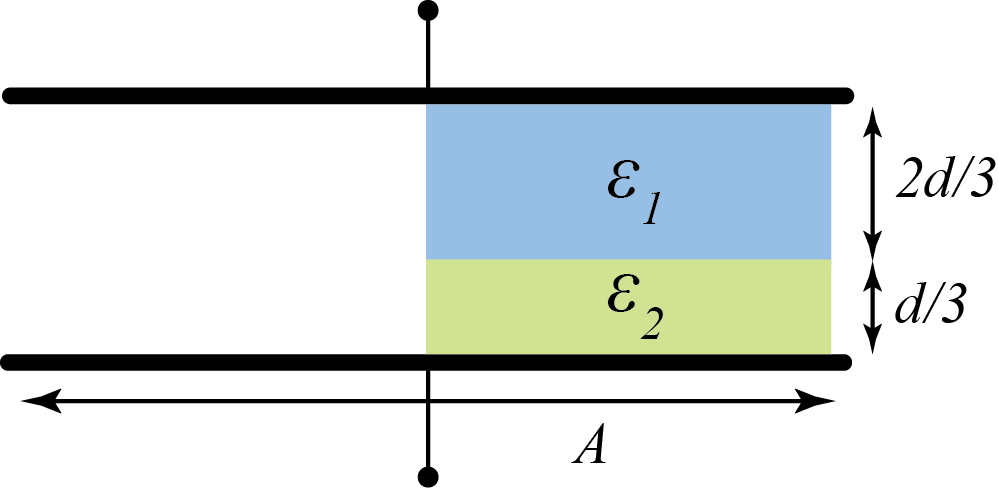
\includegraphics[height=4cm]{fig_2.png}
    \caption{Configuración Problema 2}
    \label{fig:fig_2}
\end{figure}

\begin{enumerate}[a)]
    \item Determine la nueva capacidad del condensador con los bloques dieléctricos en su interior.
    \item Calcule como se distribuye la carga en las placas conductoras.
\end{enumerate}